\chapter{计算机程序}
计算机程序是一段指令,用来告诉计算机如何执行任务。
\footnote{\url{https://www.khanacademy.org/computing/computer-programming/programming/intro-to-programming/v/programming-intro}}
\section{计算机程序有什么用}
最初的计算机大多用来做科学计算,如早期的计算机之一Z3主要用来做空气动力学中计算\footnote{\url{https://en.wikipedia.org/wiki/Z3_(computer)}}。

\begin{paperbox}{\textbf{Learning By Reading}\startwo}
阅读以下资料,了解早期计算机长什么样,用来做什么。\\
\href{http://www.computerhistory.org/timeline/computers/}{\textit{Timeline of Computer History}}
\end{paperbox}
现在的程序显然不仅限于用来计算,我们的手机、电脑中的软件、App便由一个或多个程序构成。
\begin{paperbox}{\textbf{Learning By Thinking}\starfour}
你能想到哪些程序?它们都是用来干什么的?
\end{paperbox}
\begin{paperbox}{\textbf{Learning By Reading}\startwo}
相信软件、App是大家经常听到的概念,那么程序、软件、App三者之间有什么异同呢?阅读以下材料做个大体上的了解。\\
\href{https://teamtreehouse.com/community/the-difference-between-application-program-software}{\textit{软件、程序、App三者的区别}}\\
\href{https://www.guokr.com/question/544735/}{\textit{软件和程序有区别么?区别在哪}}
\end{paperbox}
\section{编程语言}
人与人之间的交流需要自然语言(Natural language,或人类语言Human language),而与计算机交流,使用的便是编程语言。\\
编程语言与自然语言有类似之处,乔姆斯基(Chomsky)的形式语言(Formal language)理论认为,一门语言中的任何一个句子都是由数目有限的一系列语法规则生成出来的。
自然语言中的句子就相当于计算机指令,而编程语言同自然语言一样,有自己的语法规则,并且这套语法规则比起自然语言的语法更加确定、简单。\\
就像每一篇文章都是由某种自然语言写就,每一个计算机程序也是由某种编程语言实现。
\begin{paperbox}{\textbf{Learning By Reading}\starthree}
\href{https://www.quora.com/Whats-the-difference-between-natural-languages-and-programming-languages}{自然语言与编程语言之间的区别}
\end{paperbox}
\begin{paperbox}{\textbf{Learning By Reading}\starone}
阅读以下材料,进一步了解编程语言和计算机程序的联系\\
\href{https://zhidao.baidu.com/question/96230010.html}{程序和编程语言是不是一个概念}\\
简单概括起来,编程语言=语言,程序=文章。
\end{paperbox}
\subsection{机器语言、汇编语言、高级语言}
\begin{figure}[htbp]
\centering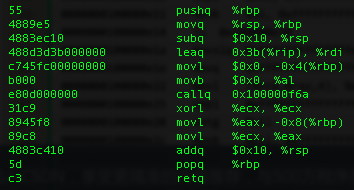
\includegraphics{image/machine_code_and_assemble.png}\\
\caption{左边一栏是机器语言,右边两栏合在一起是汇编语言}\label{fig.machine.language}
\end{figure}
直接给计算机下一个类似于“帮我做完作业”的指令显然还停留在人类的幻想之中。\\
计算机可以\textbf{\textit{直接}}执行的指令集合叫机器语言,而汇编语言是与机器语言有强烈对应关系的一种语言
\footnote{\url{https://en.wikipedia.org/wiki/Assembly_language}}
。图\ref{fig.machine.language}是机器语言和汇编语言的一个实际例子,程序的作用是输出`Hello World!'。\\
\begin{paperbox}{\textbf{Learning By Thinking}\starfour}
谈谈自己看到机器语言和汇编语言的感受。
\end{paperbox}
可以看出,机器语言很难看懂,即\textbf{可读性}很差,汇编语言虽然把机器语言变成了一个一个单词组成的句子,但实际上仍然很难看懂。
此外,不同型号的CPU使用的机器语言也可能不相同,因此,机器语言/汇编语言的\textbf{可移植性}很差。而很差的可读性也会给程序的编写和调试增加难度。\\
但机器语言/汇编语言也不是没有优点,一个优秀的汇编程序员可以写出十分高效率的汇编语言。
\begin{figure}[htb]
\centering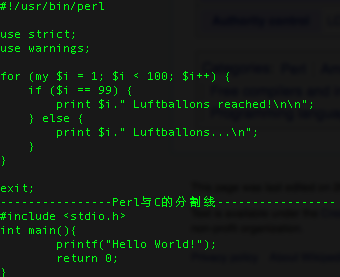
\includegraphics{image/perl_c.png}\\
\caption{下边是C,上边是Perl}\label{fig.high.level.language}
\end{figure}
\begin{figure}[htb]
\centering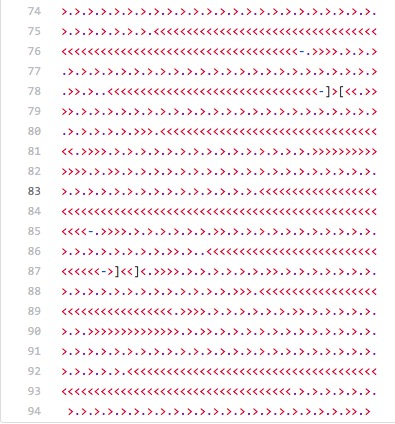
\includegraphics{image/brainfuck.png}\\
\caption{brainf**k,大神们的休闲娱乐方式$\sim$图片来源:\url{https://github.com/dotzero/brainfuck-php/blob/master/examples/99bottlesofbeer.bf}}\label{fig.brainfuck}
\end{figure}
\begin{paperbox}{\textbf{Learning By Reading}\starone}
我们经常说计算机用的是二进制,而刚才的例子里面我们看到的机器语言是用十六进制表达的,它们之间有什么联系和区别?\\
\href{https://stackoverflow.com/questions/21571709/difference-between-machine-language-binary-code-and-a-binary-file}{机器语言与二进制文件}
\end{paperbox}
高级语言是相对于低级语言的一个概念,一般来讲,它没有特别明确的定义,任何\textbf{对用户友好}且\textbf{独立于硬件}的语言都可以叫高级语言
\footnote{\url{https://www.techopedia.com/definition/3925/high-level-language-hll}}
。我们平时接触到的编程语言基本都是高级语言,比如C,Pascal,Perl,Java等。\\
高级语言不能直接被执行,必须先被转化为机器语言,我们将在下一个章节简要介绍转化的过程。\\
高级语言的一条指令通常会被转化为机器语言的多条指令,例如求一个数的平方根,用机器语言写一个
求平方根的程序需要很多指令,但在大多数高级语言中,只需要一条指令就可以完成,
这种把多条指令变成一条指令的技术叫做\textbf{抽象}
\footnote{\url{https://en.wikipedia.org/wiki/Abstraction_(software_engineering)}}
图\ref{fig.high.level.language}是C语言和Perl语言的例子。
\begin{paperbox}{\textbf{Learning By Thinking}\starfour}
谈谈自己看到高级语言的感受,与机器语言、汇编语言有什么不同?
\end{paperbox}
显而易见,高级语言更加可读。虽然我们现在还看不懂,但还是能辨认出若干英文单词来。\\
高级语言大多是为了让人们更方便地编程而设计出来的,也有一些编程语言不是为此而设计的。
比如图\ref{fig.brainfuck}便展示了一种叫brainf**k的编程语言。
\begin{paperbox}{\textbf{Learning By Reading}\starone}
如何看待brainf**k这类语言?它和汇编语言有怎样的异同和优劣?请看
\href{https://www.slant.co/versus/120/128/~assembly_vs_brainfuck}{这里}\\
从brainf**k出发哲学地看高级语言与低级语言,请看
\href{https://esolangs.org/wiki/Category_talk:Low-level}{这里}
\end{paperbox}
